\documentclass{beamer}
\mode<presentation>{
  \usetheme{Boadilla}
  \usefonttheme[onlylarge]{structurebold}
  \usefonttheme[stillsansseriflarge]{serif}
  \setbeamerfont*{frametitle}{size=\normalsize,series=\bfseries}
  % \setbeamertemplate{navigation symbols}{}
  \setbeamercovered{transparent}
}
\usepackage[english]{babel}
\usepackage[latin1]{inputenc}
\usepackage{times}
\usepackage[T1]{fontenc}
\usepackage{amsmath}
\usepackage{amssymb}
\usepackage{esint}
\usepackage{hyperref}
\usepackage{tikz}
\usepackage{xkeyval}
\usepackage{xargs}
\usepackage{verbatim}
\usepackage{listings}
\usetikzlibrary{
  arrows,
  calc,
  decorations.pathmorphing,
  decorations.pathreplacing,
  decorations.markings,
  fadings,
  positioning,
  shapes
}

\mode<handout>{
  \usepackage{pgfpages}
  \pgfpagesuselayout{4 on 1}[a4paper,landscape,border shrink=5mm]
  \setbeamercolor{background canvas}{bg=black!10}
}

\newcommand\pgfmathsinandcos[3]{%
  \pgfmathsetmacro#1{sin(#3)}%
  \pgfmathsetmacro#2{cos(#3)}%
}
\newcommand\LongitudePlane[3][current plane]{%
  \pgfmathsinandcos\sinEl\cosEl{#2} % elevation
  \pgfmathsinandcos\sint\cost{#3} % azimuth
  \tikzset{#1/.estyle={cm={\cost,\sint*\sinEl,0,\cosEl,(0,0)}}}
}
\newcommand\LatitudePlane[3][current plane]{%
  \pgfmathsinandcos\sinEl\cosEl{#2} % elevation
  \pgfmathsinandcos\sint\cost{#3} % latitude
  \pgfmathsetmacro\yshift{\cosEl*\sint}
  \tikzset{#1/.estyle={cm={\cost,0,0,\cost*\sinEl,(0,\yshift)}}} %
}
\newcommand\DrawLongitudeCircle[2][1]{
  \LongitudePlane{\angEl}{#2}
  \tikzset{current plane/.prefix style={scale=#1}}
  % angle of "visibility"
  \pgfmathsetmacro\angVis{atan(sin(#2)*cos(\angEl)/sin(\angEl))} %
  \draw[current plane] (\angVis:1) arc (\angVis:\angVis+180:1);
  \draw[current plane,dashed] (\angVis-180:1) arc (\angVis-180:\angVis:1);
}
\newcommand\DrawLatitudeCircleArrow[2][1]{
  \LatitudePlane{\angEl}{#2}
  \tikzset{current plane/.prefix style={scale=#1}}
  \pgfmathsetmacro\sinVis{sin(#2)/cos(#2)*sin(\angEl)/cos(\angEl)}
  % angle of "visibility"
  \pgfmathsetmacro\angVis{asin(min(1,max(\sinVis,-1)))}
  \draw[current plane,decoration={markings, mark=at position 0.6 with {\arrow{<}}},postaction={decorate},line width=.6mm] (\angVis:1) arc (\angVis:-\angVis-180:1);
  \draw[current plane,dashed,line width=.6mm] (180-\angVis:1) arc (180-\angVis:\angVis:1);
}
\newcommand\DrawLatitudeCircle[2][1]{
  \LatitudePlane{\angEl}{#2}
  \tikzset{current plane/.prefix style={scale=#1}}
  \pgfmathsetmacro\sinVis{sin(#2)/cos(#2)*sin(\angEl)/cos(\angEl)}
  % angle of "visibility"
  \pgfmathsetmacro\angVis{asin(min(1,max(\sinVis,-1)))}
  \draw[current plane] (\angVis:1) arc (\angVis:-\angVis-180:1);
  \draw[current plane,dashed] (180-\angVis:1) arc (180-\angVis:\angVis:1);
}
\newcommand\coil[1]{
  {\rh * cos(\t * pi r)}, {\apart * (2 * #1 + \t) + \rv * sin(\t * pi r)}
}
\makeatletter
\define@key{DrawFromCenter}{style}[{->}]{
  \tikzset{DrawFromCenterPlane/.style={#1}}
}
\define@key{DrawFromCenter}{r}[1]{
  \def\@R{#1}
}
\define@key{DrawFromCenter}{center}[(0, 0)]{
  \def\@Center{#1}
}
\define@key{DrawFromCenter}{theta}[0]{
  \def\@Theta{#1}
}
\define@key{DrawFromCenter}{phi}[0]{
  \def\@Phi{#1}
}
\presetkeys{DrawFromCenter}{style, r, center, theta, phi}{}
\newcommand*\DrawFromCenter[1][]{
  \setkeys{DrawFromCenter}{#1}{
    \pgfmathsinandcos\sint\cost{\@Theta}
    \pgfmathsinandcos\sinp\cosp{\@Phi}
    \pgfmathsinandcos\sinA\cosA{\angEl}
    \pgfmathsetmacro\DX{\@R*\cost*\cosp}
    \pgfmathsetmacro\DY{\@R*(\cost*\sinp*\sinA+\sint*\cosA)}
    \draw[DrawFromCenterPlane] \@Center -- ++(\DX, \DY);
  }
}
\newcommand*\DrawFromCenterText[2][]{
  \setkeys{DrawFromCenter}{#1}{
    \pgfmathsinandcos\sint\cost{\@Theta}
    \pgfmathsinandcos\sinp\cosp{\@Phi}
    \pgfmathsinandcos\sinA\cosA{\angEl}
    \pgfmathsetmacro\DX{\@R*\cost*\cosp}
    \pgfmathsetmacro\DY{\@R*(\cost*\sinp*\sinA+\sint*\cosA)}
    \draw[DrawFromCenterPlane] \@Center -- ++(\DX, \DY) node {#2};
  }
}
\makeatother

% not mandatory, but I though it was better to set it blank
\setbeamertemplate{headline}{}
\def\beamer@entrycode{\vspace{-\headheight}}

\tikzstyle{snakearrow} = [decorate, decoration={pre length=0.2cm,
  post length=0.2cm, snake, amplitude=.4mm,
  segment length=2mm},thick, ->]

%% document-wide tikz options and styles

\tikzset{%
  % >=latex, % option for nice arrows
  inner sep=0pt,%
  outer sep=2pt,%
  mark coordinate/.style={inner sep=0pt,outer sep=0pt,minimum size=3pt,
    fill=black,circle}%
}
\tikzset{
  % Define standard arrow tip
  >=stealth',
  % Define style for boxes
  punkt/.style={
    rectangle,
    rounded corners,
    draw=black, very thick,
    text width=8em,
    minimum height=2.5em,
    text centered},
}
\makeatletter
\newbox\@backgroundblock
\newenvironment{backgroundblock}[2]{%
  \global\setbox\@backgroundblock=\vbox\bgroup%
  \unvbox\@backgroundblock%
  \vbox to0pt\bgroup\vskip#2\hbox to0pt\bgroup\hskip#1\relax%
}{\egroup\egroup\egroup}
\addtobeamertemplate{background}{\box\@backgroundblock}{}
\makeatother

% \def\timeleft{15:00->14:55}

\title[\textbf{Cs} Raman transition]{Raman transition on single Cesium Atom}
\author{Yichao Yu}
\institute{Ni Group/Harvard}

\begin{document}

\begin{frame}{}
  \titlepage
\end{frame}

% \begin{frame}{}
%   \tableofcontents
% \end{frame}

\begin{frame}[t]{}
  \begin{columns}[t]
    \column{5cm}
    \begin{center}
      \only<1-8, 11-13, 16-> {
        \begin{tikzpicture}[scale=0.9]
          \visible<+-> {
            \draw[line width=1] (0, 0) -- (2, 0);
            \path (1, 0) node[above] {$|4', -3\rangle$};
            \draw[line width=1] (2.5, -0.2) -- (4.5, -0.2);
            \path (3.5, -.2) node[above] {$|4', -4\rangle$};
            \draw[line width=1] (0, -0.8) -- (2, -0.8);
            \path (1, -.8) node[above] {$|3', -3\rangle$};

            \draw[line width=1] (0, -5) -- (2, -5);
            \path (1, -5) node[above] {$|4, -3\rangle$};
            \draw[line width=1] (2.5, -5.2) -- (4.5, -5.2);
            \path (3.5, -5.2) node[above] {$|4, -4\rangle$};
            \draw[line width=1] (0, -7) -- (2, -7);
            \path (1, -7) node[above] {$|3, -3\rangle$};
          }

          \visible<+-> {
            \draw[line width=1,dashed,blue] (2.5, -2) -- (4.5, -2);
            \draw[line width=1,dashed,blue,<->] (2.7, -2) -- (2.7, -.2);
            \path (2.7, -1.1) node[right] {$\approx18\text{GHz}$};
            \draw[line width=1,red,->] (4.1, -5.2) -- (4.1, -2);
            \draw[line width=1,red,->] (4.1, -2) -- (1.55, -7);
          }
        \end{tikzpicture}
      }
      \only<9-10> {
        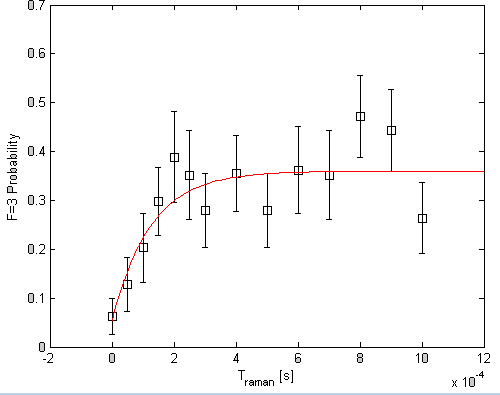
\includegraphics[width=5cm]{Scatter.png}
      }
      \only<14-15> {
        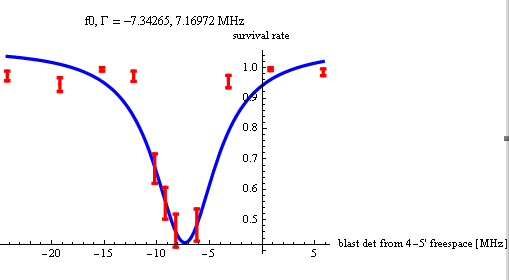
\includegraphics[width=5cm]{4_-4.png}\\
        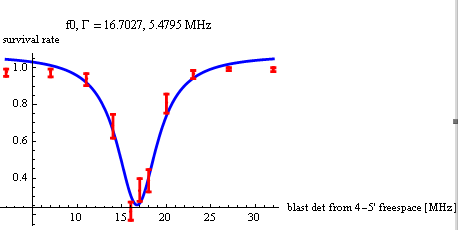
\includegraphics[width=5cm]{4_4.png}
      }
    \end{center}
    \column{6.5cm}
    \only<3-15>{
      \begin{block}{}
        \begin{itemize}
          \item<3-> Use single atom
          \item<4-> Light
            \begin{itemize}
            \item<5-> Power \visible<10->{\checkmark}
            \item<10-> Frequency \visible<12->{\checkmark}
            \end{itemize}
          \item<12-> State \visible<15->{\checkmark}
        \end{itemize}
      \end{block}
      \only<6-9>{
        \begin{itemize}
        \item<6-> Shrink size
        \item<7-> Alignment
        \item<8-> Scattering measurement
        \end{itemize}
      }
      \only<10-11>{
        \begin{itemize}
        \item<10-> Use co-propagating beams
        \item<11-> Measure beat note
        \end{itemize}
      }
      \only<13-14>{
        \begin{itemize}
        \item<13-> Dark state pumping
        \item<14-> Cycling transition Zeeman shift
        \end{itemize}
      }
    }
    \only<16->{
      \begin{center}
        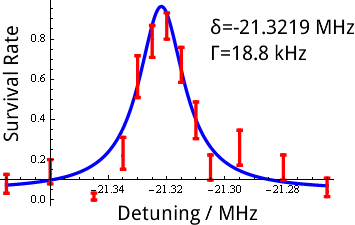
\includegraphics[width=6cm]{Raman_line.png}
      \end{center}
      \begin{block}{}
        \begin{itemize}
        \item<17->
          Zeeman shift $\approx21\text{MHz}$
        \item<18->
          Red shifted (and wider) with higher Raman intensity
        \end{itemize}
      \end{block}
    }
  \end{columns}
\end{frame}

\begin{frame}{Rabi flopping}
  \begin{columns}
    \column{6cm}
    \visible<+->{
      \begin{center}
        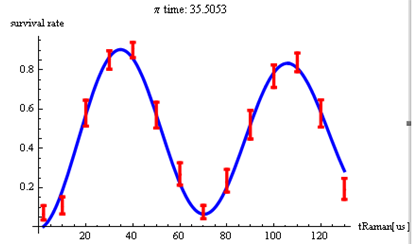
\includegraphics[width=5.5cm]{Raman_Rabi.png}
      \end{center}
    }
    \column{6cm}
    \visible<+->{
      \begin{center}
        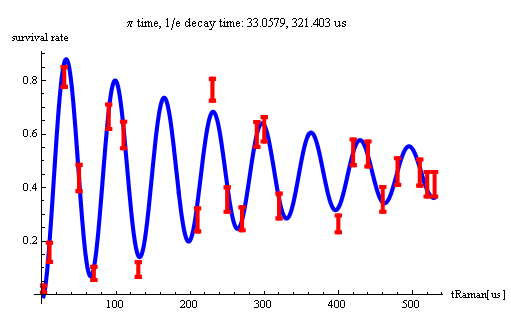
\includegraphics[width=5.5cm]{Raman_Rabi_damp.png}
      \end{center}
    }
  \end{columns}
  \visible<+-> {
    \begin{center}
      \begin{block}{Next}
        \begin{itemize}[<+->]
        \item More characterization (Power, heating, decoherence)
        \item Drive sideband
        \end{itemize}
      \end{block}
    \end{center}
  }
\end{frame}

\begin{frame}{}
\end{frame}

\begin{frame}{}
\end{frame}

\end{document}
